\documentclass[10pt,aspectratio=169,handout]{beamer}

\usepackage[utf8]{inputenc}
\usepackage[ngerman]{babel}
\usepackage{utopia}
\usetheme{Darmstadt}
\usecolortheme{default}
\usepackage{xcolor}
\usepackage{graphicx}
\usepackage{amsmath}
\usepackage{amsthm}
\usepackage{amssymb}
\usepackage{amsfonts}
\usepackage{mathtools}
\usepackage{dsfont}
\usepackage{hyperref}
\usepackage[most]{tcolorbox}
\usepackage{tikz}
\usepackage{adjustbox}
\usepackage{mathrsfs}
\usepackage{minted}
\usetikzlibrary{cd}
\usetikzlibrary{positioning}
\usetikzlibrary{calc}
\usetikzlibrary{arrows.meta}
\setbeamertemplate{theorems}[numbered]
\setbeamertemplate{navigation symbols}{}
\newtranslation[to=ngerman]{Theorem}{Satz}
\def\C{\mathbb{C}}
\def\R{\mathbb{R}}
\def\Q{\mathbb{Q}}
\def\N{\mathbb{N}}
\def\Z{\mathbb{Z}}
\def\cA{\mathcal{A}}
\definecolor{LightGray}{gray}{0.9}


\begin{document}

\title{Principles of Machine Learning: Exercise 2}
\date{19.11.2023}
\author{Alina Pollehn (3197257), Julian Litz (3362592), Manuel Hinz (3334548)\\
    Felix Göhde (3336445), Felix Lehmann (3177181), Caspar Wiswesser (3221493)\\
    Adrian Köring (3347785), Greta Günther (3326765), Linus Mallwitz (3327653)\\
    Niklas Mueller-Goldingen (3363219), Jennifer Kroppen (2783393)}

\begin{frame}
    \maketitle
\end{frame}

\section{Exercise 2.1}
\begin{frame}
    \frametitle{Task 2.1.1-2 :: Loading}
    Instead of removing the outliers, its easier to keep the inliers:
    \inputminted[bgcolor=LightGray,fontsize=\small]{python}{code/filter-outliers.py}

    Maximum Likelihood Estimation of a Gaussian via empirical mean and covariance:
    \inputminted[bgcolor=LightGray,fontsize=\small]{python}{code/gaussian-mle.py}
\end{frame}

\begin{frame}
    \frametitle{Task 2.1.3 :: Predictions}
    Conditional Probability of a Gaussian:
    \inputminted[bgcolor=LightGray,fontsize=\small]{python}{code/predict-gaussian.py}
    
    \begin{columns}
        \begin{column}{0.5\textwidth}
        \begin{center}
            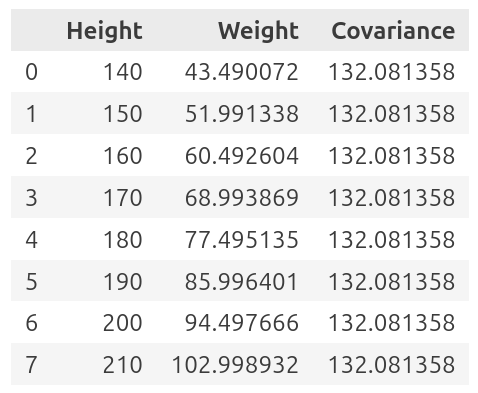
\includegraphics[width=0.7\textwidth]{images/predictions.png}
        \end{center}
        \end{column}
        \begin{column}{0.5\textwidth}  
        \begin{figure}
            \centering
            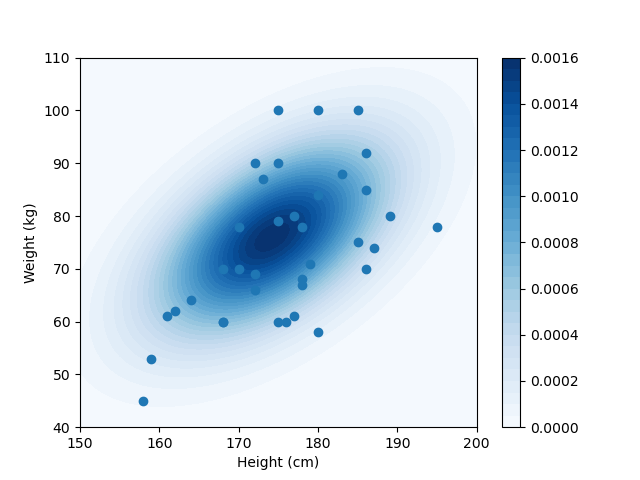
\includegraphics[width=0.7\textwidth]{images/gaussian.png}
            \caption{Estimated PDF and given data}
            \end{figure}
        \end{column}
    \end{columns}
\end{frame}

\begin{frame}
    \frametitle{Task 2.1.3 :: Pondering}

    \begin{itemize}
        \item[+] Results seem plausible -- can mostly judge around the mean
        \item[-] Fixed variance doesn't match expectations
        \begin{itemize}
            \item maybe taller people $\rightarrow$ more variance?
            \item there are more average sized people $\rightarrow$ maybe more variance? 
        \end{itemize}
        \item[-] Cube-Square-Law / BMI suggests a non-linear / quadratic relationship?
        \item[-]    Plausibility? Test-Set and more 'human-readable' metrics!
    \end{itemize}
\end{frame}

\section{2.2}
\begin{frame}
    \frametitle{Task 2.2.1 :: Loading}
    \begin{columns}
    \begin{column}{0.6\textwidth}
        \inputminted[bgcolor=LightGray,fontsize=\small]{python}{code/myspace-pre.py}
    \end{column}
    \begin{column}{0.4\textwidth}
        \begin{figure}
            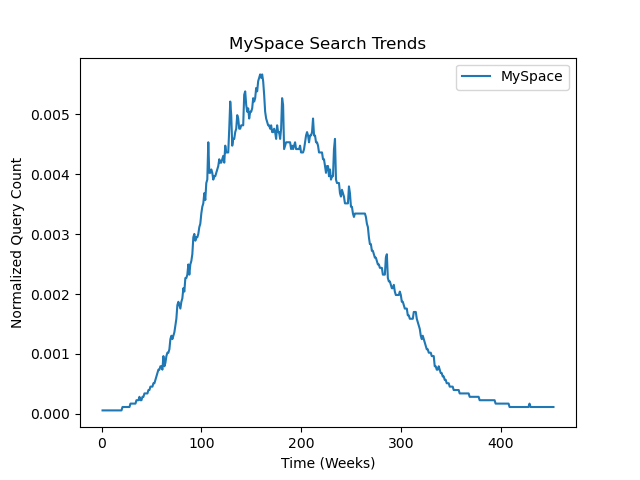
\includegraphics[width=\textwidth]{images/myspace.png}
        \end{figure}
    \end{column}
    \end{columns}
\end{frame}

\begin{frame}
    \frametitle{Task 2.2.2 :: A more efficient way to calculate partial derivatives (1)}

    Goal: Fitting a Weibull distribution $f(t|\alpha,\beta)=\frac{\alpha}{\beta} \left(\frac{t}{\beta}^{\alpha-1}e^{-\left(\frac{t}{\beta}^\alpha\right)}\right)$
    While our data is given as a histogram, our derivatives are expressed in terms of a set of numbers.
    We therefore calculate $N=\sum_{i=1}^n h_i$ and rewrite our sums in terms of $h_i$:
    \[\frac{\partial L}{\partial\beta}=\frac{\alpha}{\beta}\left(\sum_{i=1}^N \left(\frac{d_i}{\beta}\right)^\alpha-N\right)=\frac{\alpha}{\beta}\left(\sum_{i=1}^n \sum_{j=1}^{h_i}\underbrace{\left(\frac{t_{i,j}}{\beta}\right)^\alpha}_{\text{constant for fixed }i}-N\right)=\frac{\alpha}{\beta}\left(\sum_{i=1}^n h_i\left(\frac{t_i}{\beta}\right)^\alpha-N\right)\]
\end{frame}

\begin{frame}
    \frametitle{Task 2.2.2 :: A more efficient way to calculate partial derivatives (2)}
    We can rewrite all of our derivatives in this way to get:
    \[ \frac{\partial L}{\partial \alpha} = \frac{N}{\alpha}-N\log\beta+\sum_{i=1}^n h_i \log t_i-\sum_{i=1}^n h_i \left(\frac{t_i}{\beta}\right)^\alpha \log\frac{t_i}{\beta}\]
    \[\frac{\partial^2 L}{\partial \alpha^2}=-\frac{N}{\alpha^2}-\sum_{i=1}^n h_i \left(\frac{t_i}{\beta}\right)^\alpha \left(\log \frac{t_i}{\beta}\right)^2\] 
    \[\frac{\partial^2 L}{\partial \beta^2} = \frac{\alpha}{\beta^2}\left(N-(\alpha+1)\sum_{i=1}^n h_i \left(\frac{t_i}{\beta}\right)^\alpha\right)\] 
    \[ \frac{\partial^2 L}{\partial \alpha \partial \beta} = \frac{1}{\beta} \sum_{i=1}^n h_i\left(\frac{t_i}{\beta}\right)^\alpha +\frac{\alpha}{\beta}\sum_{i=1}^n h_i\left(\frac{t_i}{\beta}\right)^\alpha \log \frac{t_i}{\beta}-\frac{N}{\beta}\]
\end{frame}

\begin{frame}
    \frametitle{Task 2.2.2 :: Results}
    Our MLE implementation yields \[\alpha\approx 2.809\]
    \[\beta\approx 215.429\]
        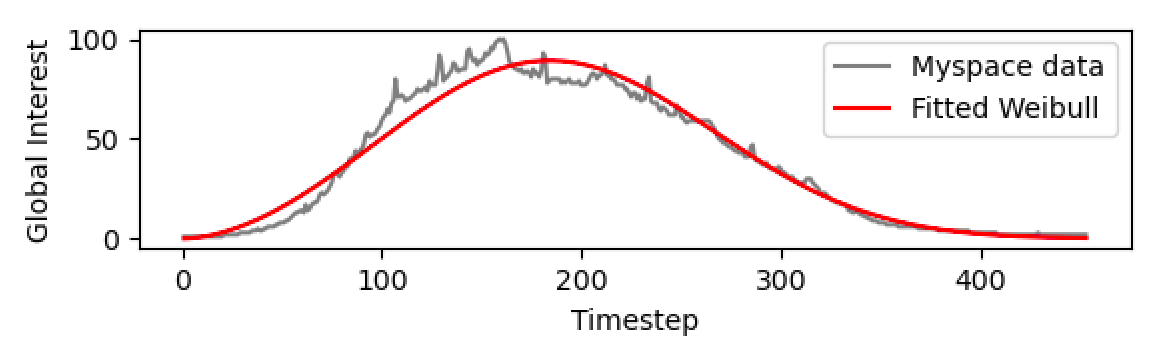
\includegraphics[width=\textwidth]{images/Fitted_Weibull_T2.png}
\end{frame}

\section{2.3}
\begin{frame}
    \frametitle{Task 2.3 :: Scipy CurveFit}
    \inputminted[bgcolor=LightGray,fontsize=\small]{python}{code/curve-fit.py}

    \begin{columns}
        \begin{column}{0.7\textwidth}
            \begin{itemize}
                \item mostly works just like that
                \item could have also scaled the data (see 2.5) \\
                        instead of adding the amplitude parameter
                \item $A=17459.4$, $\alpha=2.731$, $\beta=211.024$
            \end{itemize}
        \end{column}
    
        \begin{column}{0.3\textwidth}
            \begin{figure}
                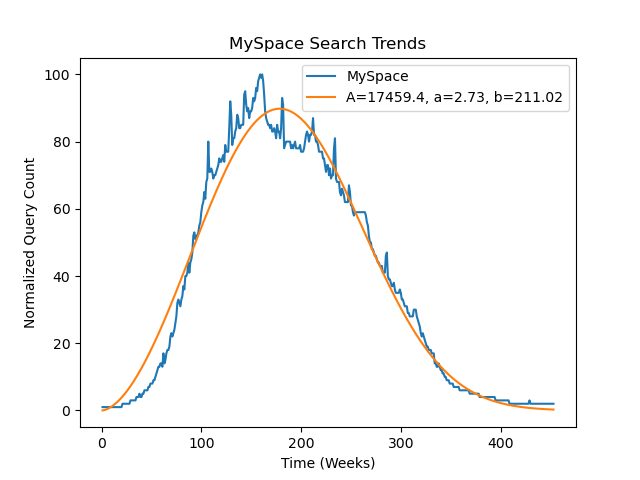
\includegraphics[width=\textwidth]{images/scicurvefit.png}
            \end{figure}
        \end{column}
        \end{columns}
    
\end{frame}

\section{2.4}
\begin{frame}
    \frametitle{Task 2.4 :: Theory}

    \begin{enumerate}
        \item Idea: Fitting a multinomial distribution to our histogram:
        \begin{align*}
            h(x_1,\dots,x_n)&=N!\prod_{i}\frac{p_i^{x_i}}{x_i!}\\
            p_i(\theta_1,\theta_2)&=\begin{cases}
                F(t_i)-F(t_{i-1} & i>0\\
                F(t_i) & i=0 
            \end{cases})
        \end{align*}
        \item Use a iterative weighted least squares scheme:\[\sum_i w_i (x_i-Np_i(\theta_1,\theta_2))^2\]
        \item Scipy's least squares only wants a function which computes the residual of a single data point ($h_i, t_i$): \[\sqrt{w_i}(x_i-Np_i(\theta_1,\theta_2))\]  
    \end{enumerate}

\end{frame}

\begin{frame}
    \frametitle{Task 2.4 :: Results}
    \vspace{-5mm}
    \inputminted[bgcolor=LightGray,fontsize=\small]{python}{code/weibull_histrogram.py}
    yields 
    \vspace{-5mm}
    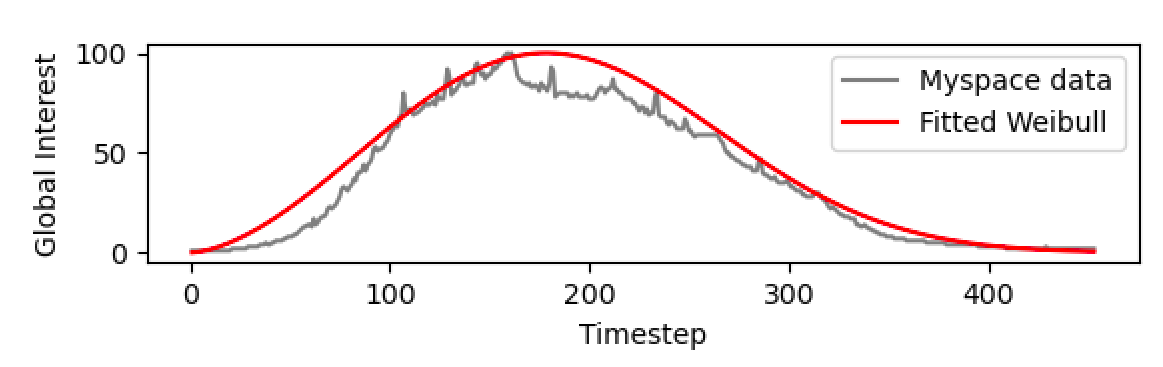
\includegraphics[width=\textwidth]{images/Fitted_Weibull_T4.png}
    \vspace{-5mm}
    \begin{itemize}
        \item $\alpha=2.646$  and $\beta=213.454$
        \item Observation: Choosing a arbitrary ftol $\in [10^{-16},10^{-10}]$ yields the result above, while choosing a higher tolerance ($10^{-4}$) yields $2.646, 213.454$. In this case 
        it does not make a significant difference (both in speed and accuracy) which (reasonable) tolerance we use.
    \end{itemize}

\end{frame}

\section{2.5}
\begin{frame}
    \frametitle{Task 2.5 :: Scipy Minimize}
    \inputminted[bgcolor=LightGray,fontsize=\small]{python}{code/minimize-kl.py}

    \begin{columns}
    \begin{column}{0.7\textwidth}
        \begin{itemize}
            \item $\alpha=2.87$, $\beta=215.91$
            \item Bounds are important, but also not: $[-\infty, \infty]$ works, too
            \item Feels odd anyway, because a gradient method optimizing \\ 
                    1 $\rightarrow$ 2.8 shouldn't come near 0 anyway
            \item[$\Rightarrow$] Adding bounds just change the algorithm underneath
            \item Without bounds 'BFGS' is choosen and doesnt quite work
            \item 'L-BFGS-B' or 'SLSQP' without bounds works equally well
        \end{itemize}
    \end{column}

    \begin{column}{0.3\textwidth}
        \begin{figure}
            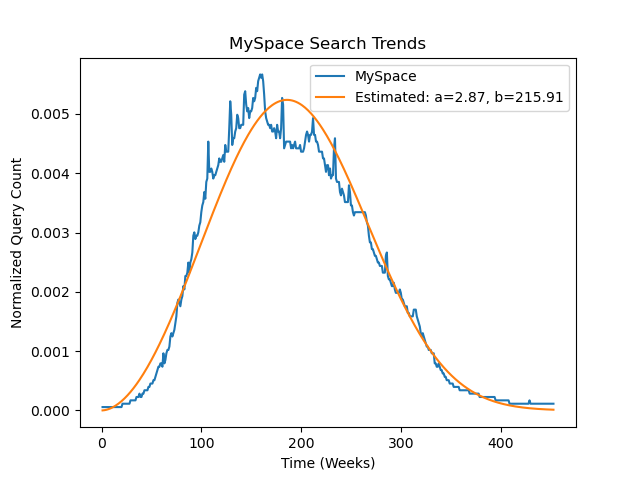
\includegraphics[width=\textwidth]{images/sciminimize.png}
        \end{figure}
    \end{column}
    \end{columns}

\end{frame}

\section{Results}

\begin{itemize}
    \item In Task 2.2, 2.3, 2.4 and 2.5 we fitted a Weibull distribution to the same dataset.

    \begin{tabular}{|c|c|c|c|c|}
        \hline
        & 2.2 & 2.3 & 2.4 & 2.5\\ \hline 
        $\alpha$ & 2.809 & 2.731 & 2.646 & 2.87\\\hline
        $\beta$ & 215.429 & 211.024 & 213.454 & 215.91\\\hline
    \end{tabular}
    \item Each task had a different way to formalize ''fitting a Weibull distribution'', therefore slightly different result are not surprising
    \item No single fit is the best, each minimizes a different loss. 
    \item Depending on the use case, it might be useful to add another random component (such as a gaussian with mean zero) to better explain small deviations from our (scaled) Weibull distribution  
\end{itemize}
\begin{figure}
    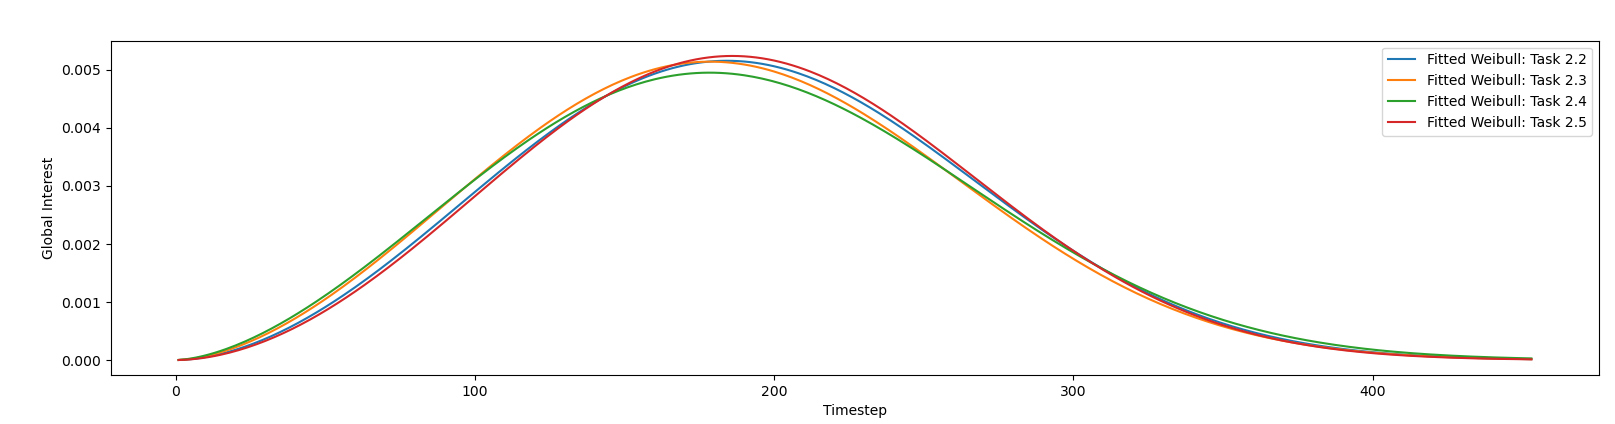
\includegraphics[width=\textwidth]{images/fitted_weibulls.png}
\end{figure}

\end{document}
